\documentclass[a4paper, 12pt]{article}

% a nice font
\usepackage{kpfonts}

% basic text stuff
\usepackage[utf8]{inputenc}
\usepackage[T1]{fontenc}

\usepackage{colortbl} % to color rows or columns of matrices

\usepackage{tikz} % main tikz package
\usepackage{tikz-network} % provides graph / network utilities (Edge, Node, etc)

\usetikzlibrary{backgrounds} % to explicitely draw in the background layer
\usetikzlibrary{calc} % to do some computations on the coordinates

% for a nicer colorscheme
\definecolor{blue}{rgb}{0.38, 0.51, 0.71} %glaucous, 97,130,181, #6182B5
\definecolor{darkblue}{RGB}{17, 42, 60} % 112A3C
\definecolor{red}{RGB}{175, 49, 39} % AF3127

\definecolor{orange}{RGB}{217, 156, 55} % D99C37
\definecolor{green}{RGB}{144, 169, 84} % 90A954
\definecolor{palegreen}{RGB}{197, 184, 104} % C5B868

\definecolor{yellow}{RGB}{250, 199, 100} % FAC764
\definecolor{brokenwhite}{RGB}{218, 192, 166} % DAC0A6
\definecolor{brokengrey}{rgb}{0.77, 0.76, 0.82} % {196,194,209}, C4C2D1


\begin{document}

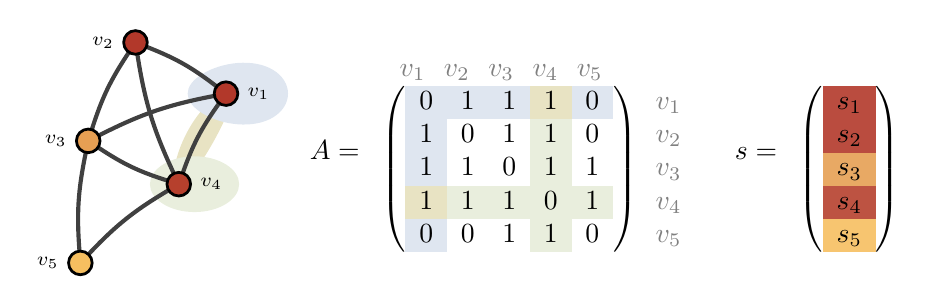
\begin{tikzpicture}[scale=0.5]
    \begin{scope}[on background layer]
        \coordinate (v1) at (4.8,4.5);
        \coordinate (v4) at (3.6,2.2);

        \fill [palegreen!40] plot [smooth cycle, tension=1] coordinates {(v1) ($ (v1) + (-0.2,-1)$) (v4) ($ (v1) + (-1,-1)$)};
        \fill [blue!20] plot [smooth cycle, tension=1] coordinates {($ (v1) + (1.2,0.6) $) ($ (v1) + (1.2,-0.6) $) ($ (v1) + (-0.6,-0.5) $) ($ (v1) + (-0.6,0.5) $)};
        \fill [green!20] plot [smooth cycle, tension=1] coordinates {($ (v4) + (1.2,0.5) $) ($ (v4) + (1.2,-0.5) $) ($ (v4) + (-0.4,-0.5) $) ($ (v4) + (-0.4,0.5) $)};
    \end{scope}

    \Vertex[x=4.8,y=4.5,size=0.3,color={178,56,42},label=$v_1$,position=right,RGB]{0}
    \Vertex[x=2.5,y=5.8,size=0.3,color={178,56,42},label=$v_2$,position=left,RGB]{1}
    \Vertex[x=1.3,y=3.3,size=0.3,color={230,159,83},label=$v_3$,position=left,RGB]{2}
    \Vertex[x=3.6,y=2.2,size=0.3,color={182,64,45},label=$v_4$,position=right,RGB]{3}
    \Vertex[x=1.1,y=0.2,size=0.3,color={246,191,96},label=$v_5$,position=left,RGB]{4}
    \Edge[,bend=-8](0)(1)
    \Edge[,bend=-8](0)(2)
    \Edge[,bend=-8](0)(3)
    \Edge[,bend=-8](1)(2)
    \Edge[,bend=-8](1)(3)
    \Edge[,bend=-8](2)(3)
    \Edge[,bend=-8](2)(4)
    \Edge[,bend=-8](3)(4)

    \node (matrix) at (12,3) {$
        A = \begin{array}{l}
            \color{gray}{~~ v_1 ~~ v_2 ~~ v_3 ~~ v_4 ~~ v_5} \\
            \left(
                \begin{array}{>{\columncolor{blue!20}}ccc>{\columncolor{green!20}}cc}
    	            \rowcolor{blue!20} 0  & 1 & 1 & \cellcolor{palegreen!40} 1 & 0 \\
    	            1 & \cellcolor{palegreen!0} 0 &\cellcolor{palegreen!0} 1 &\cellcolor{green!20} 1 &\cellcolor{palegreen!0} 0 \\
    	            1 & \cellcolor{palegreen!0}1 & \cellcolor{palegreen!0}0 &\cellcolor{green!20} 1 & \cellcolor{palegreen!0}1 \\
    	            \rowcolor{green!20}\cellcolor{palegreen!40} 1  & 1 & 1 & 0 & 1 \\
    	            \cellcolor{blue!20}0 &\cellcolor{palegreen!0} 0 &\cellcolor{palegreen!0} 1 & 1 &\cellcolor{palegreen!0} 0 \\
                \end{array}
            \right)
            \color{gray}{
                \begin{array}{c}
                    v_1 \\ v_2 \\ v_3 \\ v_4 \\ v_5
                \end{array}
            }
        \end{array}$};

    \definecolor{signal_1}{RGB}{178,56,42}
    \definecolor{signal_2}{RGB}{178,56,42}
    \definecolor{signal_3}{RGB}{230,159,83}
    \definecolor{signal_4}{RGB}{182,64,45}
    \definecolor{signal_5}{RGB}{246,191,96}

    \node (vector) at (20,3) {$
    s = \begin{array}{l}\\
            \left(
                \begin{array}{c}
                    \cellcolor{signal_1!90}s_1 \\
                    \cellcolor{signal_2!90}s_2 \\
                    \cellcolor{signal_3!90}s_3 \\
                    \cellcolor{signal_4!90}s_4 \\
                    \cellcolor{signal_5!90}s_5
                \end{array}
            \right)
        \end{array}
    $};
    
\end{tikzpicture}

\end{document}
